\section{Stakeholder, Ziele und Produktumfang}
\label{sec:Kap-6.1}

Den Begriff \textit{Stakeholder} -- für den es wie für den Begriff Requirements Engineering keine hundertprozentig adäquate deutsche Übersetzung gibt -- hatten wir in Abschnitt~1.2.2 % TODO Abschnitt~\ref{sec:Kap-1.3.2}
bereits erwähnt. Er umfasst alle Personen(gruppen), deren Interessen in irgendeiner Weise durch das zu entwickelnde Softwareprodukt berührt werden oder die Einfluss auf die Erstellung des Produkts nehmen können. Im Hinblick auf Require\-ments Engineering bedeutet das, dass diese Personen (mittelbar oder unmittelbar) Anforderungen an das Softwareprodukt stellen (können).  

Doch längst nicht alle Bedürfnisse der Stakeholder sind relevant für das konkret zu entwickelnde Softwareprodukt. Die \textbf{Stakeholder} und ihre Bedürfnisse müssen in Einklang gebracht werden mit den \textbf{(Unternehmens)Zielen}, die durch den Einsatz des Softwareprodukts erreicht werden sollen und dem Aufgabenfeld (der so genannte \textbf{Produktumfang}, engl. scope), das die zukünftige Software abdecken soll: 

\begin{itemize}[
		label={\sttpHervorhebung{$\Rightarrow$}},
		]
	\item Die Ziele, 
		\marginline{der Zirkel aus Stakeholdern, Zielen und Produktumfang}
		die mit dem Einsatz des Softwareprodukts erreicht werden sollen, sind die Grundlage für den Produktumfang. Letzterer gibt an, für welche Aufgabenbereiche das Softwareprodukt zuständig ist und für welche nicht. Abhängig vom Produktumfang sind unterschiedlich viele Gruppen von Stakeholdern vom Einsatz der Software betroffen und werden Anforderungen stellen. Die in das Softwareentwicklungsprojekt eingebundenen Stakeholder beeinflussen aber wiederum die Definition der Ziele, damit auch den Produktumfang, damit die Menge der Stakeholder usw. \cite[44]{rob13} nennt diesen Abhängigkeitszyklus „the trinity of scope, stakeholders, and goals“. 
\end{itemize}

In der Praxis können Ziele, Stakeholder und Produktumfang daher nicht isoliert voneinander betrachtet werden -- im Rahmen dieses Lerntexts werden wir es zugunsten der systematischen Darstellung in den folgenden Abschnitten trotzdem so handhaben. In der Praxis wird man mit einem der drei Aspekte beginnen -- meistens hat der Auftraggeber zumindest eine grobe Vorstellung vom gewünschten Produktumfang -- und alle drei iterativ so lange anpassen, bis sie stimmig sind. Unabhängig davon, in welcher Reihenfolge und wie stark parallelisiert die Bestimmung von Zielen, Stakeholdern und Produktumfang in einem Softwareentwicklungsprojekt stattfindet: Vor der systematischen Ermittlung von Anforderungen an das Softwareprodukt sollten diese drei Analysen abgeschlossen oder zumindest weit fortgeschritten sein. Andernfalls ist die Wahrscheinlichkeit hoch, dass für die Ermittlung zu vieler, und auch später nicht berücksichtigter Anforderungen unnötig Ressourcen investiert wurden.

Abbildung~\ref{fig:stakeholder_ziele_produktumfang_anfoderungen} zeigt den Zusammenhang zwischen Zielen, Stakeholdern und Produkt\-umfang auf der einen Seite und den Anforderungen auf der anderen Seite:

\begin{itemize}
	\item Die \textbf{\sttpHervorhebung{Bedürfnisse}} der Stakeholder \textbf{\sttpHervorhebung{manifestieren sich in den Anforderungen}}. Insofern bilden die Bedürfnisse der Stakeholder die Basis für die Anforderungen.
	\item Der \textbf{\sttpHervorhebung{Produktumfang}} ist der \textbf{\sttpHervorhebung{Rahmen}}, in den die Anforderungen passen müssen. Die Anforderungen müssen also zu dem vom Produktumfang definierten Aufgabenbereich gehören.
	
	\pagebreak %%% für Druck
	
	\item Die \textbf{\sttpHervorhebung{Ziele}} sind der \textbf{\sttpHervorhebung{Maßstab für die Relevanz}} der Anforderungen. Das bedeutet, dass jede im Softwareentwicklungsprojekt berücksichtigte Anforderung zur Erfüllung mindestens eines der Ziele des Projekts beitragen muss.
\end{itemize}

\begin{figure}[!t]
	\vspace{\baselineskip} %%% für Druck
	\centering
	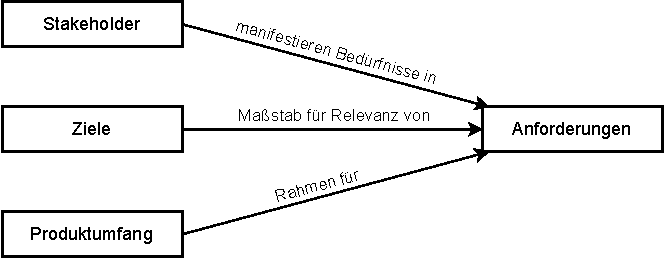
\includegraphics{Bilder/Kapitel-6/begriffe-version1.pdf}
	\caption{Stakeholder, Ziele, Produktumfang und Anforderungen}
	\label{fig:stakeholder_ziele_produktumfang_anfoderungen}
\end{figure}

Beispiel aus einer IT-fernen Lebenswelt: Der römische Staatsmann Cato der Ältere (234-149 v. Chr.) soll alle seine Reden im Senat -- unabhängig vom Thema -- mit dem Ausspruch beendet haben: „Im Übrigen bin ich der Meinung, dass Karthago zerstört werden muss“. In dieser Anekdote ist die Zerstörung Karthagos (in der Antike ein einflussreicher Stadtstaat in Nordafrika und Gegner des Römischen Reichs) ein Bedürfnis des Stakeholders Cato, das als Anforderung „Karthago muss zerstört werden“ dokumentiert werden könnte. In einer Senatssitzung, die sich mit der Verbesserung landwirtschaftlicher Methoden beschäftigt, steht eine solche Anforderung komplett abseits des Themas. In einer Senatssitzung, die sich mit den Beziehungen zwischen dem Römischen Reich und anderen Reichen beschäftigt, würde man sie kontrovers diskutieren. Die identische Anforderung befindet sich in dem einen Fall also außerhalb, in dem anderen Fall innerhalb des definierten Aufgabenbereichs des Senats. Betrachten wir den letzteren Fall. Die Relevanz der Anforderung misst sich an den Zielen des entsprechenden Vorhabens. Wenn das Ziel des römischen Senats die Aushandlung von Bündnissen mit anderen Reichen ist, sollte Catos Anforderung der Zerstörung Karthagos besser unberücksichtigt bleiben, da sie nicht zur Erfüllung des Ziels beiträgt. Wie es endete zwischen Cato und Karthago beschreibt \linebreak 
{\small [\url{https://de.wikipedia.org/wiki/Ceterum_censeo_Carthaginem_esse_delendam}]}.

In den folgenden Abschnitten werden wir uns mit den Themen Stakeholder, Ziele und Produktumfang und ihrem Einfluss auf die Anforderungsermittlung detaillierter beschäftigen. 